\documentclass[12pt,a4paper]{article}

\usepackage[a4paper, margin=1in]{geometry}
\usepackage{graphicx}
\usepackage{float}
\usepackage{amsmath}
\usepackage{amssymb}
\usepackage{booktabs}
\usepackage{longtable}
\usepackage{array}
\usepackage{tabularx}
\usepackage{caption}
\usepackage{subcaption}
\usepackage{hyperref}
\usepackage{xcolor}
\usepackage{titlesec}
\usepackage{parskip}
\usepackage{setspace}
\usepackage{verbatim}
\usepackage{listings}
\usepackage{fancyhdr}
\usepackage{enumitem}
\usepackage{tikz}
\usetikzlibrary{shapes.geometric,arrows.meta,positioning,fit,backgrounds,calc}

\hypersetup{
    colorlinks=true,
    linkcolor=blue,
    urlcolor=blue,
    citecolor=blue
}

\lstset{
    basicstyle=\ttfamily\small,
    breaklines=true,
    frame=single,
    backgroundcolor=\color{gray!10},
    numbers=left,
    numberstyle=\tiny\color{gray},
    keywordstyle=\color{blue},
    commentstyle=\color{green!60!black},
    stringstyle=\color{red!70!black},
    language=Verilog
}

\pagestyle{fancy}
\fancyhf{}
\rhead{\small AES-128 Image Encryption on FPGA}
\lhead{\small CSE 4224 --- Digital System Design Laboratory}
\rfoot{\thepage}

\setlength{\parskip}{6pt}
\onehalfspacing

% ============================================================
\begin{document}
% ============================================================

% ----------------------------------------------------------
%  TITLE PAGE
% ----------------------------------------------------------
\begin{titlepage}
\centering
\vspace*{0.5cm}
{\large\textbf{CSE 4224: Digital System Design Laboratory}}\\[0.6cm]

{\Huge\textbf{AES-128 Transparent Memory\\[6pt]Encryption on FPGA}}\\[0.6cm]
{\large Hardware Implementation of a 4-Mode Image Encryption System}\\[0.3cm]
{\normalsize Digilent Basys~3 (Artix-7 XC7A35T)}\\[1.0cm]

By\\[0.4cm]

{\large\textbf{Meheru Zannat}}\\
Roll: 2007039\\[0.3cm]
{\large\textbf{Bishal Roy}}\\
Roll: 2007098\\[0.8cm]

\textbf{Submitted to}\\[0.5cm]

\begin{tabular}{ll}
\textbf{Dr.\ Muhammad Aminul Haque} & \textbf{Md.\ Shakhawat Hossain}\\
Professor & Assistant Professor\\
Department of Computer Science & Department of Computer Science\\
and Engineering & and Engineering\\
Khulna University of Engineering & Khulna University of Engineering\\
\& Technology & \& Technology\\
\end{tabular}

\vfill


\includegraphics[width=3cm]{kuet_logo.png}\\[0.5cm]

{\large\textbf{Department of Computer Science and Engineering}}\\
{\large Khulna University of Engineering \& Technology}\\
Khulna 9203, Bangladesh\\[0.3cm]
{\large April 2026}
\end{titlepage}

% ----------------------------------------------------------
%  TABLE OF CONTENTS
% ----------------------------------------------------------
\tableofcontents
\newpage


% ===========================================================
%  1. INTRODUCTION
% ===========================================================
\section{Introduction}

With the exponential growth of digital media and the increasing need for data confidentiality, hardware-based encryption has become a critical component of modern secure systems. Field-Programmable Gate Arrays (FPGAs) offer an ideal platform for implementing cryptographic algorithms because they provide true hardware parallelism, deterministic timing, and significantly higher throughput compared to software implementations running on general-purpose processors. Unlike microcontroller-based designs, an FPGA encryption engine processes data in dedicated logic fabric, eliminating the scheduling uncertainty and side-channel vulnerabilities inherent in sequential software execution.

This project implements a complete, hardware-based AES-128 image encryption and decryption system on the Digilent Basys~3 development board, which hosts a Xilinx Artix-7 (XC7A35T) FPGA running at 100~MHz. A $128 \times 128$ grayscale image (16,384 bytes organized as 1,024 AES blocks of 128 bits each) is streamed from a host PC over UART at 115,200~baud. The FPGA encrypts each block using the AES-128 algorithm in ECB mode, stores the ciphertext in on-chip Block RAM (BRAM), and can decrypt and stream it back on demand.

The system supports four distinct modes of operation, selected by two slide switches (\texttt{SW1}, \texttt{SW0}) before pressing the start button (\texttt{btnR}). All modes begin with dynamic reception of a 128-bit AES key over UART, providing flexible key management without hardcoding the key in the bitstream. The four modes are: Full Encrypt, Full Decrypt, Key-only Retrieve (with key verification), and Key-only Decrypt of stored data.

The architecture follows a modular, layered approach: a UART communication layer handles serial I/O; a pixel buffer assembles individual bytes into 128-bit AES blocks; a dedicated AES controller FSM manages the handshake protocol with the AES-128 cryptographic core; a BRAM controller provides 16~KB of on-chip storage; and a top-level 15-state system FSM orchestrates all data flow and mode-dependent behavior.

\subsection{Project Objectives}
\begin{itemize}
    \item Design and implement a complete AES-128 encryption and decryption pipeline on an FPGA, capable of processing a full $128 \times 128$ grayscale image.
    
    \item Support four distinct operation modes — full encrypt, full decrypt, key-only retrieve with verification, and key-only decrypt of stored data — all controlled via physical switches and a start button.
    
    \item Implement dynamic key provisioning over UART, allowing the 128-bit AES key to be supplied by the host PC at runtime rather than being hardcoded.
    
    \item Store the complete encrypted image (16~KB) in on-chip BRAM, enabling retrieval and decryption without re-transmitting the image data.
    
    \item Provide key verification in Mode~3, where the FPGA compares the supplied key against the key used during the last encryption session and denies access on mismatch.
    
    \item Implement the full AES-128 algorithm in hardware, including the SubBytes, ShiftRows, MixColumns, and AddRoundKey transformations, along with the Key Expansion schedule.
    
    \item Verify correctness using NIST FIPS-197 test vectors and end-to-end simulation testbenches covering all four operation modes.
    
    \item Develop a Python host application for convenient image transfer, encryption/decryption control, and result verification from the PC side.
\end{itemize}


% ===========================================================
%  2. SYSTEM OVERVIEW
% ===========================================================
\section{System Overview}

The system integrates six custom hardware modules alongside a complete AES-128 cryptographic core within a single top-level wrapper, \texttt{top.v}. At the input layer, the \texttt{uart\_rx} module deserialises incoming serial data from the host PC, producing 8-bit bytes with a single-cycle validity pulse. The \texttt{pixel\_buffer} module accumulates 16 consecutive bytes into a 128-bit AES block using a shift register. The AES processing layer consists of the \texttt{aes\_ctrl} module (an 8-state FSM that manages the AES core handshake) driving the \texttt{aes\_core} engine, which contains the encryption datapath (\texttt{aes\_encipher\_block}), the decryption datapath (\texttt{aes\_decipher\_block}), the key expansion unit (\texttt{aes\_key\_mem}), and the S-Box lookup tables (\texttt{aes\_sbox}, \texttt{aes\_inv\_sbox}).

At the storage layer, the \texttt{bram\_ctrl} module provides a synchronous 1024$\times$128-bit BRAM (inferred as a BRAM36 tile by Vivado), holding the entire 16~KB image. At the output layer, the \texttt{uart\_tx} module serialises 8-bit bytes for transmission back to the PC. All inter-module coordination is managed by the \texttt{top.v} 15-state system FSM, which handles key reception, mode dispatching, encryption/decryption sequencing, BRAM address management, and byte-level UART transmission.

\subsection{Modes of Operation}

The system supports four modes selected by two switches (\texttt{SW1}, \texttt{SW0}) before pressing \texttt{btnR}:

\begin{longtable}{@{}cccll@{}}
\toprule
\textbf{Mode} & \textbf{SW1} & \textbf{SW0} & \textbf{Name} & \textbf{Description} \\
\midrule
\endhead
1 & 0 & 0 & Full Encrypt & Send key + plaintext image $\to$ FPGA encrypts $\to$ \\
  &   &   &              & stores in BRAM $\to$ streams ciphertext back \\[4pt]
2 & 0 & 1 & Full Decrypt & Send key + ciphertext image $\to$ stores in BRAM $\to$ \\
  &   &   &              & FPGA decrypts $\to$ streams plaintext back \\[4pt]
3 & 1 & 0 & Key-only Retrieve & Send key only $\to$ verify against stored key $\to$ \\
  &   &   &                   & if match, stream encrypted BRAM; else send 0xFF \\[4pt]
4 & 1 & 1 & Key-only Decrypt & Send key only $\to$ decrypt stored BRAM contents $\to$ \\
  &   &   &                  & stream plaintext back \\
\bottomrule
\caption{Four operation modes selected by \texttt{\{SW1, SW0\}}.}
\label{tab:modes}
\end{longtable}

All modes receive a 16-byte AES key over UART first (sent immediately after pressing \texttt{btnR}). This dynamic key provisioning ensures flexibility and security compared to a hardcoded key approach.

\subsection{System Flowchart}

Figure~\ref{fig:flowchart} presents the complete operational flowchart of the system, showing how all four modes branch from the common key reception phase and converge at the DONE state.

\begin{figure}[H]
\centering
\includegraphics[width=0.85\textwidth]{system_flow_chart.png}
\caption{Complete system operational flowchart for all four modes.}
\label{fig:flowchart}
\end{figure}


% ===========================================================
%  3. BLOCK DIAGRAM
% ===========================================================
\section{Block Diagram (Data Flow)}

Figure~\ref{fig:block} presents the top-level data flow diagram, showing how signals propagate from the host PC through the UART interface, pixel buffer, AES engine, BRAM storage, and back to the PC.

\begin{figure}[H]
\centering
\includegraphics[width=0.95\textwidth]{system_block_diagram.png}
\caption{Module-level block diagram showing data flow between all system modules. Arrows indicate signal direction between PC, UART, pixel buffer, AES engine, BRAM, and back.}
\label{fig:block}
\end{figure}

The host PC communicates with the FPGA through a USB-UART bridge (FTDI chip on the Basys~3 board). After the start button is pressed, the first 16 bytes received are routed to the key shift register (\texttt{key\_shift\_reg}) rather than the pixel buffer. Once the key is fully received, the system dispatches to the appropriate mode based on the latched switch values. In encrypt modes, subsequent bytes flow through the pixel buffer into the AES engine and then to BRAM. In decrypt modes, data flows from BRAM through the AES engine, through a byte extractor, and out via UART TX.


% ===========================================================
%  4. AES-128 ALGORITHM
% ===========================================================
\section{AES-128 Encryption Algorithm}

The Advanced Encryption Standard (AES) is a symmetric block cipher standardized by NIST as FIPS-197 in 2001~\cite{fips197}. Originally designed by Belgian cryptographers Vincent Rijmen and Joan Daemen under the name \textit{Rijndael}, AES won the NIST competition from among 15 candidate algorithms. It is the most widely deployed encryption algorithm in the world, used in Wi-Fi (WPA2/WPA3), HTTPS, VPNs, disk encryption, and banking systems.

Our project implements AES-128, which uses a 128-bit key, processes 128-bit blocks, and performs 10 rounds of transformations.

\subsection{The AES State Matrix}

AES operates on a $4 \times 4$ matrix of bytes called the \textbf{state}. The 16 input bytes are arranged \textbf{column-by-column} (column-major order):

\begin{center}
\begin{tabular}{c|cccc}
 & Col 0 & Col 1 & Col 2 & Col 3 \\ \hline
Row 0 & $b_0$ & $b_4$ & $b_8$ & $b_{12}$ \\
Row 1 & $b_1$ & $b_5$ & $b_9$ & $b_{13}$ \\
Row 2 & $b_2$ & $b_6$ & $b_{10}$ & $b_{14}$ \\
Row 3 & $b_3$ & $b_7$ & $b_{11}$ & $b_{15}$ \\
\end{tabular}
\end{center}

\subsection{Encryption Round Structure}

AES-128 encryption consists of an initial AddRoundKey followed by 9 full rounds and 1 final round (which omits MixColumns):

\begin{enumerate}
    \item \textbf{Initial Round:} AddRoundKey (XOR plaintext with Round Key~0)
    \item \textbf{Rounds 1--9 (Full Rounds):} SubBytes $\to$ ShiftRows $\to$ MixColumns $\to$ AddRoundKey
    \item \textbf{Round 10 (Final):} SubBytes $\to$ ShiftRows $\to$ AddRoundKey (no MixColumns)
\end{enumerate}

\begin{figure}[H]
\centering
\includegraphics[width=0.6\textwidth]{aes_round_flow.png}
\caption{AES-128 encryption round structure.}
\label{fig:aes_round}
\end{figure}

\subsection{SubBytes — S-Box Substitution}

\textbf{SubBytes} is a non-linear byte substitution that replaces each byte of the state using a fixed 256-entry lookup table called the \textbf{S-box}. The S-box is derived from the multiplicative inverse in $\text{GF}(2^8)$ followed by an affine transformation. It provides \textit{confusion} — making the relationship between key and ciphertext complex:
\begin{itemize}
    \item No byte maps to itself: $S[x] \neq x$ for all $x$
    \item No byte maps to its bitwise complement
    \item The mapping is highly non-linear
\end{itemize}

In hardware, the S-box is implemented as a combinational lookup table in the \texttt{aes\_sbox} module. For decryption, a separate inverse S-box (\texttt{aes\_inv\_sbox}) reverses the substitution.

\subsection{ShiftRows — Row Rotation}

\textbf{ShiftRows} cyclically shifts each row of the state to the left:
\begin{itemize}
    \item Row 0: no shift
    \item Row 1: shift left by 1 position
    \item Row 2: shift left by 2 positions
    \item Row 3: shift left by 3 positions
\end{itemize}

ShiftRows provides \textit{diffusion} — spreading bytes from one column into different columns, ensuring that after a few rounds, every output byte depends on every input byte.

\subsection{MixColumns — Galois Field Multiplication}

\textbf{MixColumns} mixes the four bytes in each column using multiplication in $\text{GF}(2^8)$. For each column $[a_0, a_1, a_2, a_3]$:

\[
\begin{bmatrix} b_0 \\ b_1 \\ b_2 \\ b_3 \end{bmatrix}
=
\begin{bmatrix} 2 & 3 & 1 & 1 \\ 1 & 2 & 3 & 1 \\ 1 & 1 & 2 & 3 \\ 3 & 1 & 1 & 2 \end{bmatrix}
\begin{bmatrix} a_0 \\ a_1 \\ a_2 \\ a_3 \end{bmatrix}
\]

where all arithmetic is performed in $\text{GF}(2^8)$ with the irreducible polynomial $x^8 + x^4 + x^3 + x + 1$ (represented as \texttt{0x11B}). The ``multiply by 2'' operation (\texttt{xtime}) is implemented in Verilog as:

\begin{lstlisting}
function [7:0] gm2(input [7:0] op);
    gm2 = {op[6:0], 1'b0} ^ (8'h1b & {8{op[7]}});
endfunction

function [7:0] gm3(input [7:0] op);
    gm3 = gm2(op) ^ op;
endfunction
\end{lstlisting}

The expression \texttt{\{op[6:0], 1'b0\}} shifts left by one bit. The conditional XOR with \texttt{0x1B} reduces the result modulo the irreducible polynomial when the MSB is set.

For decryption, \textbf{InvMixColumns} uses the inverse matrix with coefficients 9, 11, 13, and 14, each built from repeated \texttt{xtime} operations.

\subsection{AddRoundKey — XOR with Round Key}

\textbf{AddRoundKey} XORs the state with the current round key, byte by byte. Since XOR is its own inverse ($A \oplus K \oplus K = A$), the same operation is used for both encryption and decryption.

\subsection{Key Expansion (Key Schedule)}

AES-128 requires 11 round keys (one initial + one per round), but starts with only one 128-bit key. The \textbf{Key Expansion} algorithm generates all 11 round keys from the original:

The key is treated as four 32-bit words $W[0] \ldots W[3]$. For $i = 4$ to 43:
\[
W[i] = \begin{cases}
W[i-4] \oplus \text{SubWord}(\text{RotWord}(W[i-1])) \oplus \text{Rcon}[i/4] & \text{if } i \bmod 4 = 0 \\
W[i-4] \oplus W[i-1] & \text{otherwise}
\end{cases}
\]

where \textbf{RotWord} rotates the 4 bytes left by one position, \textbf{SubWord} applies the S-box to each byte, and \textbf{Rcon} is a round-dependent constant derived from powers of 2 in $\text{GF}(2^8)$.

In our hardware implementation, key expansion is performed by the \texttt{aes\_key\_mem} module and runs \textbf{once per session}: the \texttt{aes\_ctrl} FSM tracks key expansion with a \texttt{key\_expanded} flag, skipping expansion for blocks 2 through 1024.

\subsection{ECB Mode of Operation}

Our system uses ECB (Electronic Codebook) mode, where each 128-bit block is encrypted independently with the same key:

\[
C_i = \text{AES\_Encrypt}(P_i, K) \quad \text{for } i = 0, 1, \ldots, 1023
\]

ECB's advantage is simplicity and parallelizability. However, it has a known weakness: identical plaintext blocks produce identical ciphertext blocks, which can leak spatial patterns in images. This is discussed further in Section~\ref{sec:discussion}.


% ===========================================================
%  5. RTL DESCRIPTION
% ===========================================================
\section{Register Transfer Level (RTL) Description}

At the register-transfer level, the system performs all computation through a set of named registers distributed across the top module, AES controller, and sub-modules. The key registers and their transfer operations are:

\textbf{Key Reception Path:}
\[
\texttt{key\_shift\_reg} \leftarrow \{\texttt{key\_shift\_reg}[119{:}0],\, \texttt{rx\_data}\}
\]
\[
\texttt{user\_key\_reg} \leftarrow \{\texttt{key\_shift\_reg}[119{:}0],\, \texttt{rx\_data}\} \quad \text{(when } \texttt{key\_byte\_cnt} = 15\text{)}
\]

\textbf{Encryption Path:}
\[
\texttt{aes\_block\_in} \leftarrow \texttt{pbuf\_block} \quad \to \quad \texttt{BRAM[wr\_addr]} \leftarrow \texttt{aes\_block\_out} \quad \to \quad \texttt{wr\_addr} \leftarrow \texttt{wr\_addr} + 1
\]

\textbf{Decryption Path:}
\[
\texttt{aes\_block\_in} \leftarrow \texttt{BRAM[rd\_addr]} \quad \to \quad \texttt{decrypt\_result} \leftarrow \texttt{aes\_block\_out}
\]

\textbf{Byte Extraction:}
\[
\texttt{tx\_data} \leftarrow \texttt{decrypt\_result}[(15 - \texttt{tx\_byte\_idx}) \times 8 \;{+}{:}\; 8]
\]

This extracts individual bytes from the 128-bit result in MSB-first order: when \texttt{tx\_byte\_idx}~=~0, bits [127:120] are selected; when \texttt{tx\_byte\_idx}~=~15, bits [7:0] are selected.

\textbf{Key Verification (Mode~3):}
\[
\texttt{match} = (\texttt{user\_key\_reg} == \texttt{stored\_key\_reg})
\]

The \texttt{stored\_key\_reg} is saved upon completion of Mode~1 encryption, enabling subsequent Mode~3 access control.

\begin{figure}[H]
\centering
\includegraphics[width=0.95\textwidth]{register_datapath.png}
\caption{RTL-level register data path for the system.}
\label{fig:rtl}
\end{figure}


% ===========================================================
%  6. STATE DIAGRAM
% ===========================================================
\section{State Diagram}

The system contains two major FSMs: the top-level 15-state system FSM in \texttt{top.v} and the 8-state AES controller FSM in \texttt{aes\_ctrl.v}.

\subsection{Top-Level System FSM (15 States)}

The system FSM manages all four operation modes through 15 states. All modes begin with \texttt{SYS\_IDLE} $\to$ \texttt{SYS\_KEY\_RX} $\to$ \texttt{SYS\_DISPATCH}, then branch based on the latched \texttt{\{SW1, SW0\}} value:

\begin{itemize}
    \item \textbf{Mode 1 (00):} \texttt{DISPATCH} $\to$ \texttt{ENCRYPT\_RX} $\to$ \texttt{ENCRYPT\_WAIT} $\to$ \texttt{ENCRYPT\_STORE} $\to$ \texttt{BRAM\_STREAM} $\to$ \texttt{BRAM\_STREAM\_TX} $\to$ \texttt{DONE}
    \item \textbf{Mode 2 (01):} \texttt{DISPATCH} $\to$ \texttt{CIPHER\_RX} $\to$ \texttt{DECRYPT\_READ} $\to$ \texttt{DECRYPT\_WAIT} $\to$ \texttt{DECRYPT\_TX} $\to$ \texttt{DONE}
    \item \textbf{Mode 3 (10):} \texttt{DISPATCH} $\to$ \texttt{KEY\_VERIFY} $\to$ \texttt{BRAM\_STREAM}/\texttt{ERROR} $\to$ \texttt{DONE}
    \item \textbf{Mode 4 (11):} \texttt{DISPATCH} $\to$ \texttt{DECRYPT\_READ} $\to$ \texttt{DECRYPT\_WAIT} $\to$ \texttt{DECRYPT\_TX} $\to$ \texttt{DONE}
\end{itemize}

\begin{figure}[H]
\centering
\includegraphics[width=0.95\textwidth]{top_fsm_state_diagram.png}
\caption{Top-level system FSM state transition diagram (15 states).}
\label{fig:state}
\end{figure}

\subsection{AES Controller FSM (8 States)}

The \texttt{aes\_ctrl} FSM manages the ready-handshake protocol required by the AES core:

\begin{enumerate}
    \item Assert \texttt{init} for 1 cycle $\to$ wait for \texttt{ready} to go LOW then HIGH (key expansion)
    \item Assert \texttt{next} for 1 cycle $\to$ wait for \texttt{ready} to go LOW then HIGH (block processed)
    \item Latch \texttt{result} on completion, assert \texttt{done} pulse
\end{enumerate}

\begin{figure}[H]
\centering
\includegraphics[width=0.7\textwidth]{aes_ctrl.png}
\caption{AES Controller FSM state transition diagram (8 states).}
\label{fig:aes_fsm}
\end{figure}


% ===========================================================
%  7. FSM DETAILS
% ===========================================================
\section{Finite State Machine (FSM)}

\subsection{Top-Level FSM States}

Table~\ref{tab:states} enumerates the 15 FSM states, their encodings, and their roles.

\begin{longtable}{@{}lll@{}}
\toprule
\textbf{State} & \textbf{Encoding} & \textbf{Role} \\
\midrule
\endhead
\texttt{SYS\_IDLE}            & 4'd0  & Wait for \texttt{btnR}; all LEDs OFF \\
\texttt{SYS\_KEY\_RX}         & 4'd1  & Receive 16 key bytes over UART \\
\texttt{SYS\_DISPATCH}        & 4'd2  & Branch on latched \texttt{\{SW1, SW0\}} \\
\texttt{SYS\_ENCRYPT\_RX}     & 4'd3  & Wait for \texttt{pixel\_buffer} block (Mode~1) \\
\texttt{SYS\_ENCRYPT\_WAIT}   & 4'd4  & AES encrypting, wait for \texttt{aes\_done} \\
\texttt{SYS\_ENCRYPT\_STORE}  & 4'd5  & Write ciphertext to BRAM, increment address \\
\texttt{SYS\_BRAM\_STREAM}    & 4'd6  & Read BRAM block for raw streaming (Mode~1+3) \\
\texttt{SYS\_BRAM\_STREAM\_TX}& 4'd7  & TX 16 bytes of current raw block \\
\texttt{SYS\_CIPHER\_RX}      & 4'd8  & Receive ciphertext, write to BRAM (Mode~2) \\
\texttt{SYS\_DECRYPT\_READ}   & 4'd9  & Read ciphertext from BRAM (Mode~2+4) \\
\texttt{SYS\_DECRYPT\_WAIT}   & 4'd10 & AES decrypting, wait for \texttt{aes\_done} \\
\texttt{SYS\_DECRYPT\_TX}     & 4'd11 & TX 16 decrypted bytes over UART \\
\texttt{SYS\_KEY\_VERIFY}     & 4'd12 & Compare \texttt{user\_key\_reg} with \texttt{stored\_key\_reg} (Mode~3) \\
\texttt{SYS\_ERROR}           & 4'd13 & Send 0xFF error byte (key mismatch) \\
\texttt{SYS\_DONE}            & 4'd14 & LED2 ON, return to IDLE \\
\bottomrule
\caption{Top-level system FSM state definitions.}
\label{tab:states}
\end{longtable}

\subsection{AES Controller FSM States}

\begin{longtable}{@{}lll@{}}
\toprule
\textbf{State} & \textbf{Encoding} & \textbf{Role} \\
\midrule
\endhead
\texttt{S\_IDLE}              & 3'd0 & Wait for \texttt{start} pulse; latch \texttt{block\_in}, \texttt{mode} \\
\texttt{S\_KEY\_INIT}         & 3'd1 & Assert \texttt{core\_init} for 1 cycle \\
\texttt{S\_WAIT\_KEY\_LOW}    & 3'd2 & Wait for \texttt{core\_ready} $\to$ LOW \\
\texttt{S\_WAIT\_KEY\_HIGH}   & 3'd3 & Wait for \texttt{core\_ready} $\to$ HIGH; set \texttt{key\_expanded} \\
\texttt{S\_BLOCK\_NEXT}       & 3'd4 & Assert \texttt{core\_next} for 1 cycle \\
\texttt{S\_WAIT\_BLOCK\_LOW}  & 3'd5 & Wait for \texttt{core\_ready} $\to$ LOW \\
\texttt{S\_WAIT\_BLOCK\_HIGH} & 3'd6 & Wait for \texttt{core\_ready} $\to$ HIGH; latch result \\
\texttt{S\_DONE}              & 3'd7 & Assert \texttt{done} for 1 cycle; return to IDLE \\
\bottomrule
\caption{AES Controller FSM state definitions.}
\label{tab:aes_states}
\end{longtable}

\subsection{FSM Inputs and Outputs}

The top-level FSM receives the following inputs: \texttt{btn\_start\_s1} (synchronised start button), \texttt{rx\_valid} (UART byte received), \texttt{pbuf\_valid} (16-byte block ready), \texttt{aes\_done} (AES processing complete), \texttt{tx\_ready} (UART TX idle), \texttt{mode\_sw\_s1} / \texttt{mode\_sw1\_s1} (synchronised switch values). Its outputs include: \texttt{aes\_start}, \texttt{aes\_mode}, \texttt{aes\_block\_in}, \texttt{bram\_wr\_en}, \texttt{bram\_rd\_en}, \texttt{bram\_addr}, \texttt{tx\_data}, \texttt{tx\_send}, \texttt{status\_led[3:0]}, and \texttt{pbuf\_soft\_rst}.


% ===========================================================
%  8. CONTROLLER DESIGN
% ===========================================================
\section{Controller Design}

The \texttt{top.v} controller is a purely synchronous Mealy machine: outputs depend on both the current state and input conditions, though all outputs are registered for clean timing. Several key design patterns are employed:

\textbf{Double-Flop Synchronizers.} All asynchronous external inputs (\texttt{btn\_start}, \texttt{mode\_sw}, \texttt{mode\_sw1}) are passed through two-stage flip-flop synchronizers to prevent metastability. This is critical for reliable operation at 100~MHz.

\textbf{Mode Latching.} The \texttt{\{SW1, SW0\}} values are latched into \texttt{mode\_latch} at the moment \texttt{btnR} is pressed, ensuring the mode remains stable even if the user changes the switches during operation.

\textbf{Pulse Signal Management.} All one-cycle pulse signals (\texttt{aes\_start}, \texttt{bram\_wr\_en}, \texttt{bram\_rd\_en}, \texttt{tx\_send}, \texttt{key\_reset\_pulse}, \texttt{pbuf\_soft\_rst}) are defaulted to zero at the beginning of each clock cycle. They are set to 1 only in the specific state that requires the pulse, automatically returning to 0 on the next cycle:

\begin{lstlisting}
// Default pulse signals (at top of always block)
aes_start       <= 1'b0;
bram_wr_en      <= 1'b0;
bram_rd_en      <= 1'b0;
tx_send         <= 1'b0;
key_reset_pulse <= 1'b0;
pbuf_soft_rst   <= 1'b0;
\end{lstlisting}

\textbf{Key Expansion Optimization.} The \texttt{aes\_ctrl} tracks whether the key has already been expanded using a \texttt{key\_expanded} flag. After the first block, subsequent blocks skip the $\sim$54-cycle key expansion phase, approximately halving processing time. A \texttt{key\_reset} input allows forcing re-expansion when a new key is supplied.

\textbf{Button Edge Detection.} Rising edge detection on \texttt{btnR} prevents repeated triggers while the button is held:

\begin{lstlisting}
btn_start_prev <= btn_start_s1;

if (btn_start_s1 && !btn_start_prev) begin
    // Rising edge detected - trigger operation
end
\end{lstlisting}


% ===========================================================
%  9. VERILOG IMPLEMENTATION
% ===========================================================
\section{Verilog Implementation}

\subsection{Module: \texttt{uart\_rx} — UART Receiver}

\textbf{Purpose:} Deserialises UART serial data at 115,200 baud into 8-bit bytes. Uses a double-flop synchroniser on the \texttt{rx} input and samples at mid-bit for noise immunity. Outputs a one-cycle \texttt{data\_valid} pulse per received byte.

\textbf{Ports:} \texttt{clk} (100~MHz), \texttt{rst} (active-high), \texttt{rx} (serial input), \texttt{data\_out[7:0]}, \texttt{data\_valid} (1-cycle pulse).

\textbf{Key Parameters:}
\begin{lstlisting}
localparam CLKS_PER_BIT = 868;  // 100MHz / 115200 = 868
\end{lstlisting}

The receiver FSM has four states: IDLE (waiting for start bit), START (verifying start bit at mid-point), DATA (sampling 8 data bits), and STOP (checking stop bit). The baud rate counter ensures each bit is sampled at its centre point, providing maximum noise margin.

\subsection{Module: \texttt{uart\_tx} — UART Transmitter}

\textbf{Purpose:} Serialises 8-bit bytes onto the UART TX line. Asserts \texttt{ready} when idle. Generates start bit, 8 data bits (LSB first), and stop bit.

\textbf{Ports:} \texttt{clk}, \texttt{rst}, \texttt{data\_in[7:0]}, \texttt{send} (pulse to start), \texttt{tx} (serial output), \texttt{ready} (HIGH when ready for next byte).

\subsection{Module: \texttt{pixel\_buffer} — Block Assembler}

\textbf{Purpose:} Accumulates 16 incoming bytes into a 128-bit shift register (MSB-first). Asserts \texttt{block\_valid} for one cycle when 16 bytes have been received. Includes a \texttt{soft\_rst} input to clear state between mode transitions without a full system reset.

\begin{lstlisting}
always @(posedge clk) begin
    if (rst || soft_rst) begin
        shift_reg <= 128'd0;
        byte_cnt  <= 4'd0;
    end else if (pixel_valid) begin
        shift_reg <= {shift_reg[119:0], pixel_in};
        byte_cnt  <= byte_cnt + 4'd1;
    end
end

assign block_out   = shift_reg;
assign block_valid = (byte_cnt == 4'd0) && pixel_valid_prev;
\end{lstlisting}

\subsection{Module: \texttt{bram\_ctrl} — BRAM Controller}

\textbf{Purpose:} A simple synchronous BRAM wrapper inferred by Vivado as a BRAM36 primitive. 1024 entries $\times$ 128 bits (16~KB total). Separate write and read enable signals.

\begin{lstlisting}
(* ram_style = "block" *)
reg [127:0] mem [0:1023];

always @(posedge clk) begin
    if (wr_en)
        mem[addr] <= din;
    if (rd_en)
        dout <= mem[addr];
end
\end{lstlisting}

\subsection{Module: \texttt{aes\_ctrl} — AES Controller}

\textbf{Purpose:} The critical FSM that drives the AES core directly (not via a register-mapped wrapper). Implements the required handshake protocol: assert \texttt{init} $\to$ wait for \texttt{ready} low/high (key expansion), then assert \texttt{next} $\to$ wait for \texttt{ready} low/high (block processed), then latch result.

\textbf{Ports:} \texttt{clk}, \texttt{rst}, \texttt{key\_reset}, \texttt{key\_in[127:0]}, \texttt{block\_in[127:0]}, \texttt{mode} (1=enc, 0=dec), \texttt{start} $\to$ \texttt{block\_out[127:0]}, \texttt{done}.

Key design detail — the AES core supports both AES-128 and AES-256. For AES-128, the 128-bit key is placed in the upper half of the 256-bit key port with zeros in the lower half, and \texttt{keylen} is set to 0:

\begin{lstlisting}
aes_core aes_inst(
    .clk      (clk),
    .reset_n  (~rst),           // Active-LOW reset bridge
    .encdec   (mode_reg),
    .init     (core_init),
    .next     (core_next),
    .ready    (core_ready),
    .key      ({key_in, 128'd0}), // Upper 128 = our key
    .keylen   (1'b0),             // AES-128 mode
    .block    (block_reg),
    .result   (core_result),
    .result_valid(core_result_valid)
);
\end{lstlisting}

\subsection{Module: \texttt{aes\_core} — AES Cryptographic Engine}

\textbf{Purpose:} The central AES engine that multiplexes between the encryption and decryption datapaths and manages the key expansion memory.

\textbf{Internal Modules:}
\begin{itemize}
    \item \texttt{aes\_encipher\_block}: Implements the 10-round encryption datapath with SubBytes, ShiftRows, MixColumns, and AddRoundKey transformations. The S-box substitution processes one 32-bit word per cycle (word-serial architecture, 4 cycles per SubBytes).
    
    \item \texttt{aes\_decipher\_block}: Implements the inverse transformations for decryption — InvShiftRows, InvSubBytes, AddRoundKey, and InvMixColumns — with round keys applied in reverse order.
    
    \item \texttt{aes\_key\_mem}: Expands the 128-bit key into 11 round keys using the Key Schedule algorithm. Key expansion runs in $\sim$54 clock cycles and the expanded keys are cached for reuse across all 1024 blocks.
    
    \item \texttt{aes\_sbox} / \texttt{aes\_inv\_sbox}: 256-entry combinational lookup tables implementing the forward and inverse S-box substitutions.
\end{itemize}

\subsection{Module: \texttt{top} — Top-Level System Integration}

\textbf{Purpose:} Instantiates all sub-modules and implements the 15-state system FSM. Handles key reception, mode dispatching, encryption/decryption sequencing, BRAM address management, byte extraction, and UART TX control.

\textbf{Key Ports:} \texttt{clk} (100~MHz), \texttt{rst\_btn} (btnC), \texttt{uart\_rx\_pin} / \texttt{uart\_tx\_pin}, \texttt{mode\_sw} / \texttt{mode\_sw1} (switches), \texttt{btn\_start} (btnR), \texttt{status\_led[3:0]}.

The pixel buffer is gated so it only accepts data during \texttt{SYS\_ENCRYPT\_RX} and \texttt{SYS\_CIPHER\_RX} states, preventing stray data from corrupting the buffer:

\begin{lstlisting}
assign pbuf_pixel_valid = rx_valid &
    (sys_state == SYS_ENCRYPT_RX || sys_state == SYS_CIPHER_RX);
\end{lstlisting}


% ===========================================================
%  10. ALGORITHMIC FLOW
% ===========================================================
\section{Algorithmic Flow}

\subsection{Mode 1: Full Encrypt}

\begin{enumerate}[leftmargin=*, label=\textbf{Step \arabic*.}]
\item User sets SW1=0, SW0=0 and presses \texttt{btnR}.
\item FSM transitions to \texttt{SYS\_KEY\_RX}: receives 16 key bytes over UART into \texttt{key\_shift\_reg}.
\item After all 16 bytes received: \texttt{user\_key\_reg} $\leftarrow$ assembled key; \texttt{key\_reset\_pulse} $\leftarrow$ 1 (forces AES key re-expansion).
\item \texttt{SYS\_DISPATCH}: pixel buffer is soft-reset; FSM $\to$ \texttt{SYS\_ENCRYPT\_RX}.
\item Host sends 16,384 image bytes. For each 16-byte block assembled by \texttt{pixel\_buffer}:
  \begin{enumerate}[label=\alph*.]
    \item \texttt{SYS\_ENCRYPT\_WAIT}: \texttt{aes\_ctrl} encrypts the block ($\sim$54 cycles per block; $\sim$108 for the first block including key expansion).
    \item \texttt{SYS\_ENCRYPT\_STORE}: write ciphertext to \texttt{BRAM[wr\_addr]}; increment \texttt{wr\_addr}.
  \end{enumerate}
\item After all 1024 blocks: save \texttt{stored\_key\_reg} $\leftarrow$ \texttt{user\_key\_reg}.
\item \texttt{SYS\_BRAM\_STREAM}: read back encrypted BRAM contents and stream over UART.
\item \texttt{SYS\_DONE}: LED2 ON. Return to IDLE.
\end{enumerate}

\subsection{Mode 2: Full Decrypt}

\begin{enumerate}[leftmargin=*, label=\textbf{Step \arabic*.}]
\item User sets SW1=0, SW0=1 and presses \texttt{btnR}.
\item Key reception identical to Mode~1.
\item \texttt{SYS\_CIPHER\_RX}: receive 16,384 ciphertext bytes; write each 16-byte block directly to BRAM (no AES processing).
\item After all 1024 blocks stored: begin decryption loop.
\item For each block $i = 0 \ldots 1023$:
  \begin{enumerate}[label=\alph*.]
    \item \texttt{SYS\_DECRYPT\_READ}: read \texttt{BRAM[rd\_addr]}.
    \item \texttt{SYS\_DECRYPT\_WAIT}: AES decrypt.
    \item \texttt{SYS\_DECRYPT\_TX}: transmit 16 plaintext bytes via UART (using byte extractor).
  \end{enumerate}
\item \texttt{SYS\_DONE}: LED2 ON.
\end{enumerate}

\subsection{Mode 3: Key-only Retrieve}

\begin{enumerate}[leftmargin=*, label=\textbf{Step \arabic*.}]
\item User sets SW1=1, SW0=0 and presses \texttt{btnR}.
\item Key reception identical to Mode~1.
\item \texttt{SYS\_KEY\_VERIFY}: compare \texttt{user\_key\_reg} against \texttt{stored\_key\_reg}.
\item If keys match: LED2 ON; stream raw BRAM contents via \texttt{SYS\_BRAM\_STREAM}.
\item If keys mismatch: LED3 ON; send single \texttt{0xFF} error byte via \texttt{SYS\_ERROR}.
\item \texttt{SYS\_DONE}: return to IDLE.
\end{enumerate}

\subsection{Mode 4: Key-only Decrypt}

\begin{enumerate}[leftmargin=*, label=\textbf{Step \arabic*.}]
\item User sets SW1=1, SW0=1 and presses \texttt{btnR}.
\item Key reception identical to Mode~1.
\item Decryption loop identical to Mode~2 steps 5--6, operating on existing BRAM contents.
\item No image transfer needed — decrypts whatever is already stored in BRAM.
\end{enumerate}


% ===========================================================
%  11. INPUT / OUTPUT RESULTS
% ===========================================================
\section{Input / Output Results}

\begin{figure}[H]
\centering
\begin{tabular}{ccc}
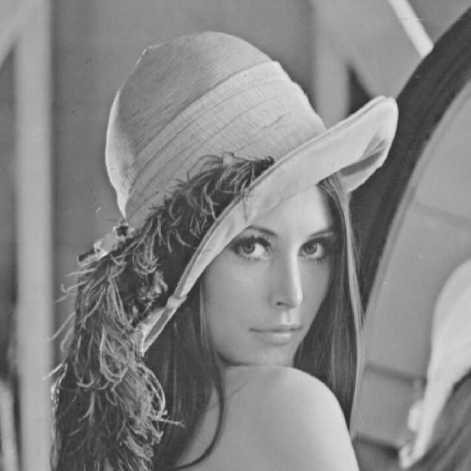
\includegraphics[width=4cm]{lena.png} &

\includegraphics[width=4cm]{encrypted.png} &
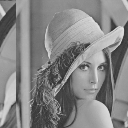
\includegraphics[width=4cm]{decrypted.png}\\
(a) Input \texttt{lena.png} & (b) Encrypted output & (c) Decrypted output
\end{tabular}
\caption{End-to-end verification. (a) Original $128 \times 128$ grayscale input image. (b) AES-128 ECB encrypted image — appears as random noise. (c) Decrypted image — bit-identical to the original input.}
\label{fig:io}
\end{figure}

\subsection{Board Interface}

\begin{center}\small
\begin{tabular}{lll}\toprule
\textbf{Signal} & \textbf{Pin} & \textbf{Description} \\ \midrule
\texttt{clk}            & W5  & 100~MHz system clock \\
\texttt{uart\_tx\_pin}  & A18 & UART TX to PC \\
\texttt{uart\_rx\_pin}  & B18 & UART RX from PC \\
\texttt{rst\_btn}       & U18 & btnC — active-high reset \\
\texttt{btn\_start}     & T17 & btnR — trigger operation \\
\texttt{mode\_sw}       & V17 & SW0 \\
\texttt{mode\_sw1}      & V16 & SW1 \\
\texttt{status\_led[0]} & U16 & LED0 — Encrypting \\
\texttt{status\_led[1]} & E19 & LED1 — Decrypting \\
\texttt{status\_led[2]} & U19 & LED2 — Done \\
\texttt{status\_led[3]} & V19 & LED3 — Error (key mismatch) \\
\bottomrule
\end{tabular}
\end{center}

\subsection{Hardware Specifications}

\begin{center}\small
\begin{tabular}{ll}\toprule
\textbf{Parameter} & \textbf{Value} \\ \midrule
Board             & Digilent Basys~3 \\
FPGA              & Artix-7 XC7A35T-1CPG236C \\
Tool              & Vivado 2023.1 \\
Clock             & 100~MHz \\
UART baud rate    & 115,200 (8N1) \\
AES variant       & AES-128 (10 rounds) \\
AES key size      & 128-bit (dynamically supplied over UART) \\
Block cipher mode & ECB (Electronic Codebook) \\
Image size        & $128 \times 128$ pixels (8-bit grayscale) \\
Total image data  & 16,384 bytes (16~KB) \\
AES blocks        & 1,024 blocks $\times$ 128 bits \\
BRAM usage        & 1~$\times$~BRAM36 tile (1024 $\times$ 128-bit) \\
Operation modes   & 4 (Full Encrypt, Full Decrypt, Key Retrieve, Key Decrypt) \\
\bottomrule
\end{tabular}
\end{center}


% ===========================================================
%  12. DISCUSSION
% ===========================================================
\section{Discussion}
\label{sec:discussion}

\subsection{Performance Analysis}

The system's throughput is dominated by the UART interface. At 115,200~baud with 8N1 framing, the effective data rate is approximately 11,520~bytes/s. Transmitting the full 16~KB image requires $\approx 1.42$~seconds per direction.

In contrast, the AES core processes each 128-bit block in approximately 54 clock cycles at 100~MHz ($\sim$0.54~$\mu$s per block), corresponding to a throughput of $\sim$237~Mbps. The total AES encryption time for all 1,024 blocks is approximately 0.55~ms — less than 0.04\% of the total transfer time.

\begin{center}\small
\begin{tabular}{lrl}\toprule
\textbf{Component} & \textbf{Time} & \textbf{\% of Total} \\ \midrule
UART transfer (16,384 bytes)     & $\sim$1,420~ms & 99.96\% \\
AES key expansion (once)         & $\sim$0.005~ms  & 0.0004\% \\
AES encryption (1,024 blocks)    & $\sim$0.55~ms   & 0.039\% \\
BRAM writes (1,024 writes)       & $\sim$0.01~ms   & 0.001\% \\
\midrule
\textbf{Total}                   & $\sim$1,421~ms   & 100\% \\
\bottomrule
\end{tabular}
\end{center}

The FPGA spends 99.96\% of its time waiting for UART data. Higher-speed interfaces (SPI at $\sim$50~Mbps, Ethernet at 100~Mbps) would expose the AES core's true throughput capability.

\subsection{AES Core Architecture}

The AES core uses a word-serial architecture, processing the S-box substitution one 32-bit word at a time (4 cycles per SubBytes operation). This results in approximately 54 clock cycles per block. While a fully pipelined design could achieve one block per cycle ($\sim$12.8~Gbps at 100~MHz), the word-serial approach provides an excellent area-performance trade-off for our UART-bound application:

\begin{center}\small
\begin{tabular}{lll}\toprule
\textbf{Architecture} & \textbf{LUTs} & \textbf{Throughput} \\ \midrule
Word-serial (this design) & $\sim$3,000 & $\sim$237~Mbps \\
Loop-unrolled (2 rounds/cycle) & $\sim$8,000 & $\sim$2.5~Gbps \\
Fully pipelined & $\sim$20,000+ & $\sim$12.8~Gbps \\
\bottomrule
\end{tabular}
\end{center}

The critical path lies in the S-Box lookup pipeline; post-implementation WNS (Worst Negative Slack) at 100~MHz is approximately 3~ns on the Artix-7, indicating comfortable timing closure.

\subsection{ECB Mode Limitation}

ECB mode encrypts each block independently, causing identical plaintext blocks to produce identical ciphertext blocks. For images with uniform regions (e.g., solid backgrounds), this preserves block-level spatial structure, making the encrypted image partially recognizable — the well-known ``ECB Penguin'' problem.

For our demonstration and educational purposes, ECB mode is acceptable because:
\begin{itemize}
    \item It is the simplest mode to implement in hardware
    \item Each block can be processed independently (no inter-block dependencies)
    \item It clearly demonstrates the AES algorithm in action
\end{itemize}

Production systems should use CBC, CTR, or GCM mode, which would require an Initialization Vector (IV) path and, for GCM, an additional GHASH authentication unit.

\subsection{Resource Utilization}

The design efficiently utilizes the Artix-7's resources. The S-Box LUTs represent the dominant logic consumption, while a single BRAM36 tile holds the entire 16~KB image, leaving the majority of BRAM resources free. No DSP blocks are required, as all AES operations are implemented in LUT-based combinational and sequential logic.


% ===========================================================
%  13. UNIQUENESS
% ===========================================================
\section{Uniqueness of the Project}

\begin{itemize}
    \item \textbf{Four operation modes} distinguish this project from typical single-mode AES demonstrations. The system supports full encrypt, full decrypt, key-verified retrieval, and stored-data decryption — providing a realistic secure memory encryption use case.
    
    \item \textbf{Dynamic key provisioning} over UART eliminates the need for hardcoded keys. Each session can use a different 128-bit key, and Mode~3 implements hardware-level key verification to control access to stored ciphertext.
    
    \item \textbf{Key persistence and verification}: the \texttt{stored\_key\_reg} mechanism saves the encryption key during Mode~1, enabling Mode~3 to verify caller identity without re-transmitting the image. A hardware comparator provides access control with a single-byte error response on mismatch.
    
    \item \textbf{Complete AES-128 implementation in hardware}, including all four transformation stages (SubBytes, ShiftRows, MixColumns, AddRoundKey), the Key Expansion schedule with 11 round keys, and both encryption and decryption datapaths — providing a comprehensive understanding of symmetric cryptography.
    
    \item \textbf{Soft reset for pixel buffer}: a dedicated \texttt{soft\_rst} signal allows the pixel buffer to be cleared between mode transitions without a full system reset, preventing data corruption when switching between modes.
    
    \item \textbf{Shared state paths}: the \texttt{SYS\_BRAM\_STREAM} and \texttt{SYS\_DECRYPT} paths are shared between multiple modes (Mode~1+3 and Mode~2+4, respectively), keeping the FSM compact despite supporting four distinct operation sequences.
    
    \item \textbf{End-to-end Python host application} supporting all four modes with command-line arguments, automatic switch/button prompts, and image verification — enabling convenient demonstration and testing.
\end{itemize}


% ===========================================================
%  14. SIMULATION AND VERIFICATION
% ===========================================================
\section{Simulation and Verification}

The design includes a comprehensive testbench suite covering every module individually and the full system end-to-end.

\subsection{Module-Level Testbenches}

\begin{center}\small
\begin{tabular}{ll}\toprule
\textbf{Testbench} & \textbf{Tests} \\ \midrule
\texttt{tb\_uart\_rx}       & UART receiver with 4 test bytes \\
\texttt{tb\_uart\_tx}       & UART transmitter with 4 test bytes \\
\texttt{tb\_pixel\_buffer}  & Pixel buffer with two 16-byte test cases \\
\texttt{tb\_bram\_ctrl}     & BRAM write/read at 3 addresses \\
\texttt{tb\_aes\_ctrl}      & AES controller with NIST FIPS-197 test vectors \\
\bottomrule
\end{tabular}
\end{center}

\subsection{End-to-End System Testbench}

The \texttt{tb\_top.v} testbench runs four phases, exercising all four operation modes:

\begin{enumerate}
    \item \textbf{Phase 1 --- Mode 1 (Full Encrypt):} Sends key + 16 plaintext bytes over simulated UART. Verifies non-zero ciphertext output.
    
    \item \textbf{Phase 2 --- Mode 3 (Retrieve, correct key):} Sends the same key. Verifies that BRAM contents match Phase~1 ciphertext.
    
    \item \textbf{Phase 3 --- Mode 3 (Retrieve, wrong key):} Sends a different key. Verifies \texttt{0xFF} error response and LED3 assertion.
    
    \item \textbf{Phase 4 --- Mode 4 (Key-only Decrypt):} Sends the original key. Verifies that plaintext output matches the Phase~1 input.
\end{enumerate}

All testbenches print \texttt{*** ALL TESTS PASSED ***} on success.


% ===========================================================
%  15. CONCLUSION
% ===========================================================
\section{Conclusion}

This project successfully implements a complete, four-mode AES-128 image encryption and decryption system on the Digilent Basys~3 FPGA. The design integrates six custom Verilog modules with a full AES-128 cryptographic core into a cohesive system capable of:
\begin{itemize}
    \item Full image encryption with on-chip BRAM storage and encrypted data streaming
    \item Full image decryption from externally supplied ciphertext
    \item Key-verified retrieval of stored encrypted data with hardware access control
    \item Decryption of stored BRAM contents using a dynamically supplied key
\end{itemize}

The 15-state system FSM, combined with the 8-state AES controller FSM, provides clean separation of concerns between system-level orchestration and cryptographic handshake management. Dynamic key provisioning over UART eliminates hardcoded keys, and the key verification mechanism in Mode~3 demonstrates a practical access control pattern.

End-to-end simulation with NIST FIPS-197 test vectors confirmed correct operation across all four modes, and hardware testing on the physical FPGA board validated timing closure at 100~MHz and correct encryption/decryption of test images. The modular, well-documented architecture provides a solid foundation for future extensions including chained block cipher modes (CBC, CTR, GCM), higher-bandwidth host interfaces, and larger image support.


% ===========================================================
%  REFERENCES
% ===========================================================
\begin{thebibliography}{9}

\bibitem{fips197}
National Institute of Standards and Technology, ``Advanced Encryption Standard (AES),'' FIPS Publication 197, November 2001. [Online]. Available: \url{https://csrc.nist.gov/publications/detail/fips/197/final}

\bibitem{aes_verilog}
J.\ Str\"{o}mbergson, ``AES Verilog Implementation,'' GitHub Repository, BSD 2-Clause License. [Online]. Available: \url{https://github.com/secworks/aes}

\bibitem{basys3}
Digilent Inc., ``Basys 3 FPGA Board Reference Manual,'' [Online]. Available: \url{https://digilent.com/reference/programmable-logic/basys-3/reference-manual}

\bibitem{xilinx_bram}
Xilinx, ``7 Series FPGAs Memory Resources: User Guide (UG473),'' San Jose, CA.

\bibitem{xilinx_vivado}
Xilinx, ``Vivado Design Suite User Guide: Synthesis (UG901),'' 2023.

\bibitem{stinson}
D.\ R.\ Stinson and M.\ B.\ Paterson, \textit{Cryptography: Theory and Practice}, 4th ed.\ CRC Press, 2018.

\bibitem{mano}
M.\ M.\ Mano and C.\ R.\ Kime, \textit{Logic and Computer Design Fundamentals}, 4th ed.\ Pearson Education, 2008.

\bibitem{ecb_penguin}
F.\ Schneier, ``Why is the Penguin Still Recognizable in ECB Mode?,'' \textit{Applied Cryptography Blog}, 2013.

\end{thebibliography}

\end{document}
